\documentclass[11pt]{article} % use larger type; default would be 10pt

\usepackage[utf8]{inputenc} % set input encoding (not needed with XeLaTeX)


\usepackage{geometry} % to change the page dimensions
\geometry{a4paper} % or letterpaper (US) or a5paper or....

\usepackage{graphicx} % support the \includegraphics command and options
\usepackage{amsmath}


\usepackage{booktabs} % for much better looking tables
\usepackage{array} % for better arrays (eg matrices) in maths
\usepackage{paralist} % very flexible & customisable lists (eg. enumerate/itemize, etc.)
\usepackage{verbatim} % adds environment for commenting out blocks of text & for better verbatim
\usepackage{subfig} % make it possible to include more than one captioned figure/table in a single float

\usepackage{fancyhdr} % This should be set AFTER setting up the page geometry
\pagestyle{fancy} % options: empty , plain , fancy
\renewcommand{\headrulewidth}{0pt} % customise the layout...
\lhead{}\chead{}\rhead{}
\lfoot{}\cfoot{\thepage}\rfoot{}

\usepackage{sectsty}
\allsectionsfont{\sffamily\mdseries\upshape} % (See the fntguide.pdf for font help)

\usepackage[nottoc,notlof,notlot]{tocbibind} % Put the bibliography in the ToC
\usepackage[titles,subfigure]{tocloft} % Alter the style of the Table of Contents
\renewcommand{\cftsecfont}{\rmfamily\mdseries\upshape}
\renewcommand{\cftsecpagefont}{\rmfamily\mdseries\upshape} % No bold!
\newcommand{\strong}[1]{\textbf{#1}}
\newcommand{\code}[1]{\texttt{#1}}
\newcommand{\st}{$^{\text{st}\ }$}
\newcommand{\nd}{$^{\text{nd}\ }$}
\newcommand{\rd}{$^{\text{rd}\ }$}
\newcommand{\nth}{$^{\text{th}\ }$}

\title{Assignment 4}
\author{Nathan Jervis}

\begin{document}
\maketitle

\section{Question 4.4}

\subsection{Part A}

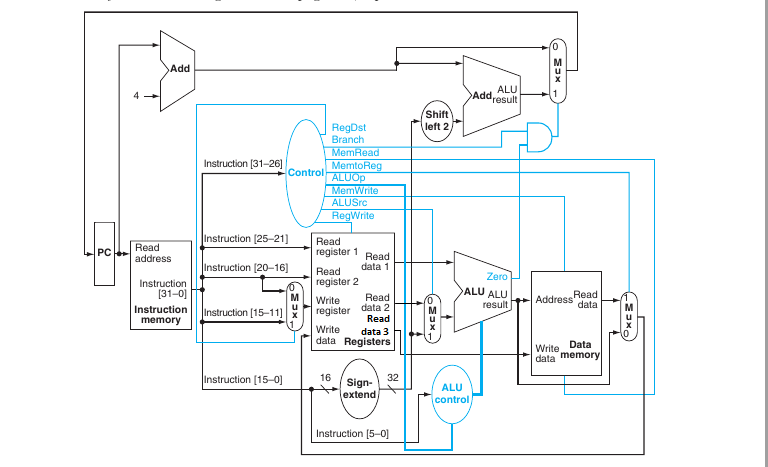
\includegraphics[width=\textwidth]{CPU3.png}

We can re-use the write register selection as the selection for a 3\rd read register. This read register is used as the write data now, instead of the 2\nd one like the previous diagram. We can make this transistion since the only opcode which currently uses that data line is \code{sw}. All we need to do is ensure that for \code{sw} the \strong{RegDst} control pin is set to 0, so the [20-16] part of the opcode is used as the write register selection. Since we've already repurposed this to read into the new 3\rd register line, it will still output the same information to the \emph{write data} section of the memory unit. \code{swr} will have \strong{RegDst} set to 1, and will therefore use the [15-11] part of the opcode to select which register to write.

Adding this new command \code{swr} requires reading from a 3\rd register, but it does not need any additional control lines, and doesn't even add new wiring to the circuit (besides what's required inside the register file to read from a 3\rd register that is). 

\subsection{Part B}

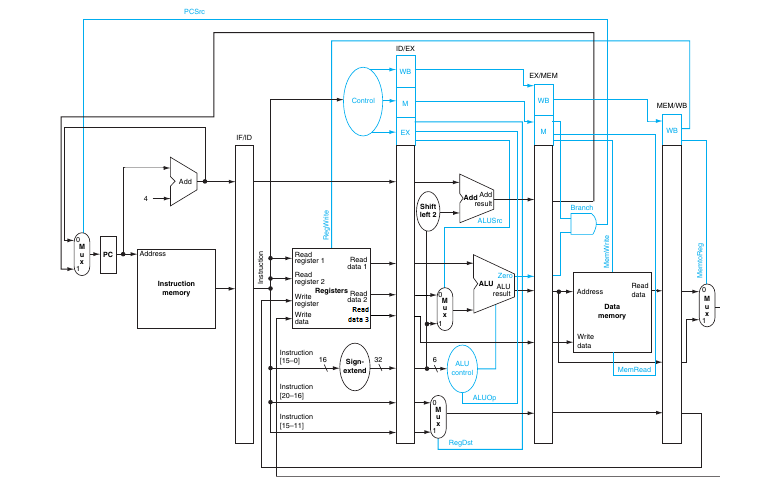
\includegraphics[width=\textwidth]{pipelineCPU2.png}

This picture is very similar to the previous one. Again the only change required is to use the write register selector to select a 3\rd  register to read from. The pipelined version also additionally requires a new spot to hold the register data between the \emph{Instruction Decode} and the \emph{Execute} stages (the one to hold the data between \emph{Execute} and \emph{Memory} already was there).

\subsection{Part C}

There are no new hazards introduced, just slightly different things to look out for. \code{lwr} has basically the same hazards as any arithmetic operation such as \code{add} (it may make a difference for optimization sake that \code{lwr} loads from memory, ie to prefetch it, but it doesn't introduce new hazards). \code{swr} is a little bit of an oddball since it now reads from a 3\rd register, and this will have to be kept in mind, but it doesn't introduce any new types of hazards, just a 3\rd spot to check for read hazards in this instruction (whereas normally it'd only check the 3\rd register for write hazards).


\section{Question 4.5}

\emph{Note: I'm assuming for these questions we're using the original CPU as in the textbook, and not the new one with \code{swr} and \code{lwr}}

\subsection{Part A}

Cross talk between \emph{RegDst} and \emph{MemWrite}, causing them to be the logical \strong{AND} of the 2 inputs. The only case when \emph{MemWrite} is 1 is when the \code{sw} opcode is used. In this case \emph{RegDst} is 0, which means with this cross-talk both \emph{RegDst} and \emph{MemWrite} will always be \code{0/false} which will cause disastrous consequences for code (as \code{sw} will never actually write it's data, and all registers which are supposed to use the 3\rd register to write to end up using the 2\nd instead, which is all \emph{r-format} instructions. In order to detect this problem the following code can be used:

\begin{verbatim}
    #load in 1 to $t0
    #immediate value functions expect RegDst to be 0, so they still work
    ori $t0, $zero, 1
    ori $t1, $zero, 2 #load in 2 to $t1
    ori $t2, $zero, 3 #load in 3 to $t2
    #add $t0 and $t1 and store in $t0
    #on an affected system, the CPU will store the result in $t1 instead
    add $t0, $t0, $t1 
    #the only possible way 2 could equal 3 would be on the broken system
    beq $t1, $t2, Fault 
\end{verbatim}

\subsection{Part B}

Cross talk between \emph{RegDst} and \emph{MemWrite}, causing them to be the logical \strong{OR} of the 2 inputs. This means that \code{sw} will now work correctly, but every instruction that sets \emph{RegDst} to 1 will also write to memory. In particular the \emph{r-format} instructions all set \emph{RegDst} to 1, so they will also write the 2\nd read register to memory (the memory location determined by the result of the operation). In order to detect this problem the following code can be used:

\begin{verbatim}
    #translated to lui and ori, both of which are I-format 
    #and not affected by this bug
    #temp is any temporary memory location that is non-zero
    li $t0, temp 
    ori $t1, $zero, 0#load 0 into t1
    sw $t1, 0($t0) #store 0 into the temp memory location
    #if the machine has this bug then it'll store 2\nd read register 
    #(which is the address of temp) into the location determined by the result 
    #(which is also the address of temp)
    #this basically means that the temp memory location now contains it's own 
    #address (which is why it must be non-zero)
    add $t2, $t1, $t0 
    lw $t2, 0($t0) #load temp back in
    beq $t2, $t1, end #check if temp is still 0
    j fault #the only way we're here is if temp was altered between sw and lw
end:   #if we reach this point we're successful, so the rest of the code can go here
\end{verbatim}

\subsection{Part C}

Cross talk between the last segment and the \emph{EX} segment of the \emph{RegWrite} causing them to be the logical \strong{AND} of the 2 inputs. This means that an instruction will only write back into the register if the instruction 2 cycles behind it is also writing back into a register (ie both are \emph{r-format} or \code{lw} instructions). Depending on the cross-talk it could also mean that the \emph{RegWrite} control bit could be affect by the instruction 2 cycles earlier. (For simplicity sake, I'm going to assume that the first 2 instructions don't get affected by the state of the \emph{RegWrite} line 2 cycles before them (which would make it completely undefined)). The following code might detect the problem:

\begin{verbatim}
    #this instruction write backs succesfully
    ori $t0, $zero, 2 #load 2 into t0
    #this instruction writes back succesfully
    ori $t1, $zero, 2 $load 2 into t1
    #this instruction fails on a problematic machine
    ori $t0, $zero, 3 #load 3 into t0
    #this is basically a nop to ensure instruction 2 works
    ori $t0, $t0, 0
    #this serves a dual purpose, it compares t0 and t1
    #and it also screws up isntruction 3 on a problem machine
    beq $t0, $t1, fault # go to fault if instruction 3 didn't work
\end{verbatim}

This code may not always work however, because depending on the implementation, it could have pipeline stalls. Simple stalls based on register usage could be avoided by adding the \code{ori $t0, $t0, 0} nop intermixed with regular \code{nop} depending on whether the instruction 2 prior should succeed or fail, but there will always be a chance that loading the instruction itself causes a cache miss, and stalls the pipeline. Also since the CPU can feel free to re-order instructions without dependencies, there is no saying that it won't re-order the program to make it execute completely differently.

\subsection{Part D}

Cross talk between the last segment and the \emph{EX} segment of the \emph{RegWrite} causing them to be the logical \strong{OR} of the 2 inputs. This means that the instruction will write back into the regiser if either it should write back, or the instruction 2 later should write back (again, depending on the nature of the cross talk, it could also be affected by instructions 2 prior, and again for simplicity I'm assuming the first 2 instructions aren't affected by the state of \emph{RegWrite} before the program starts). There is no code to detect it, since this cross-talk will only make things that aren't supposed to set RegWrite to have RegWrite set. This means \code{sw} and \code{beq}. However what gets written and where is undefined since \emph{MemToReg} and \emph{RegDst} are both undefined for those opcodes. So this means that either the result of the ALU, or the memory at the location of the result of the ALU could be written. This could be gotten around by making both of those the same (for the simple case, make them both zero), but which register they write to is undefined, and worse they could potentially write to a register that's part of the immediate value in the opcode. It would be very difficult to get around both of these problems, and considering how much any pipeline stalls would screw up the code (and since both \code{beq} and \code{sw} are very prone to causing stalls in unpredictable ways), it would be irresponsible to believe the effort would be worth it.

In short, if you believe your processor could have cross-talk here, it's not worth you time to diagnose it, go out and buy a new processor, they are super cheap.


\section{Question 4.6}

\begin{verbatim}

I1:      lw $t0, 4($s3)
I2:      addi $t0, $t0, 4
I3:      sw $t1, 0($t0)
I4:     add $t1, $t0, $t1
I5:     lw $t2, 12($s3)
I6:     addi $t2, $t2, -4
I7:     lw $t3, 8($t2)
I8:     sw $s3, 0($t1)
I9:     sw $t1, 0($t3)
\end{verbatim}

\subsection{Part A}

\begin{tabular}{c|c|c|c}
	Type & Register & Instruction 1 & Instruction 2\\\hline
	RAW & \$t0 & I1 & I2 \\
	WAW & \$t0 & I1 & I2 \\
	RAW & \$t0 & I2 & I3 \\
	WAR & \$s3 & I5 & I8 \\
	RAW & \$t1 & I3 & I4 \\
	WAW & \$t1 & I3 & I4 \\
	RAW & \$t1 & I4 & I8 \\
	WAR & \$t1 & I8 & I9 \\
	RAW & \$t2 & I6 & I7 \\
	RAW & \$t3 & I7 & I9 
\end{tabular}

\subsection{Part B}



\end{document}
